\ifx\wholebook\relax \else
% ------------------------

\documentclass[b5paper]{article}
\usepackage[nomarginpar
  %, margin=.5in
]{geometry}

\addtolength{\oddsidemargin}{-0.05in}
\addtolength{\evensidemargin}{-0.05in}
\addtolength{\textwidth}{0.1in}
\usepackage[en]{../../../prelude}

\setcounter{page}{1}

\begin{document}

\title{Binary Heaps}

\author{Xinyu LIU
\thanks{{\bfseries Xinyu LIU} \newline
  Email: liuxinyu95@gmail.com \newline}
  }

\maketitle
\fi

\markboth{Binary Heaps}{Elementary Algorithms}

\ifx\wholebook\relax
\chapter{Binary Heaps}
\numberwithin{Exercise}{chapter}
\fi

\section{Definition}
\label{introduction} \index{Binary heap}

Heaps are widely used for sorting, priority scheduling, graph algorithms, and etc.\cite{wiki-heap}. The most popular implementation uses array to represent the heap as a complete binary tree\cite{CLRS}. R.W. Floyd developed an efficient heap sort algorithm based on this idea\cite{wiki-heapsort}\cite{rosetta-heapsort}. We can implement the heap with varies data structures but not limit to array. This chapter focuses on the heaps implemented with binary trees, including leftist heap, skew heap, and splay heap\cite{okasaki-book}. A heap is either empty, or stores comparable elements that satisfy a property, and define the following operations:

\begin{enumerate}
\item \textbf{The heap property}: the top element is always the minimum;
\item \textbf{Pop}: removes the top element from the heap and maintain the heap property: the new top is still the minimum of the rest;
\item \textbf{Insert}: add a new element to the heap and maintain the heap property;
\item \textbf{Other}: operations like merge also maintain the heap property.
\end{enumerate}

Alternatively, we can define the heap that always keeps the maximum on the top. We call the heap with the minimum on the top as {\em min-heap}, the maximum on the top as {\em max-heap}. When implement heap with a tree, we can put the minimum (or the maximum) in the root. After pop, remove the root, and rebuild the tree from the sub-trees. We call the heap implemented with binary tree as {\em binary heap}.

\section{Binary heap by array}
\label{ibheap} \index{binary heap by array} \index{complete binary tree}

The first implementation is to represent the complete binary tree with array. The complete binary tree is `almost' full. The full binary tree of depth $k$ contains $2^k - 1$ nodes. We can number every node top-down, from left to right as 1, 2, ..., $2^k -1$. The node number $i$ in a complete binary tree is located at the same position in the full binary tree. The leaves only appear in the bottom layer, or the second last layer. \Cref{fig:tree-array-map} shows a complete binary tree and the array. The $i$-th cell in array corresponds to a node, its parent maps to the $\lfloor i/2 \rfloor$-th cell; the left sub-tree maps to the $2i$-th cell, and the right sub-tree maps to the $(2i + 1)$-th cell. If any sub-tree maps to an index out of the array bound, then the sub-tree does not exist (i.e. leaf node). We can define the map as below (index starts from 1):

\begin{figure}[htbp]
\centering
   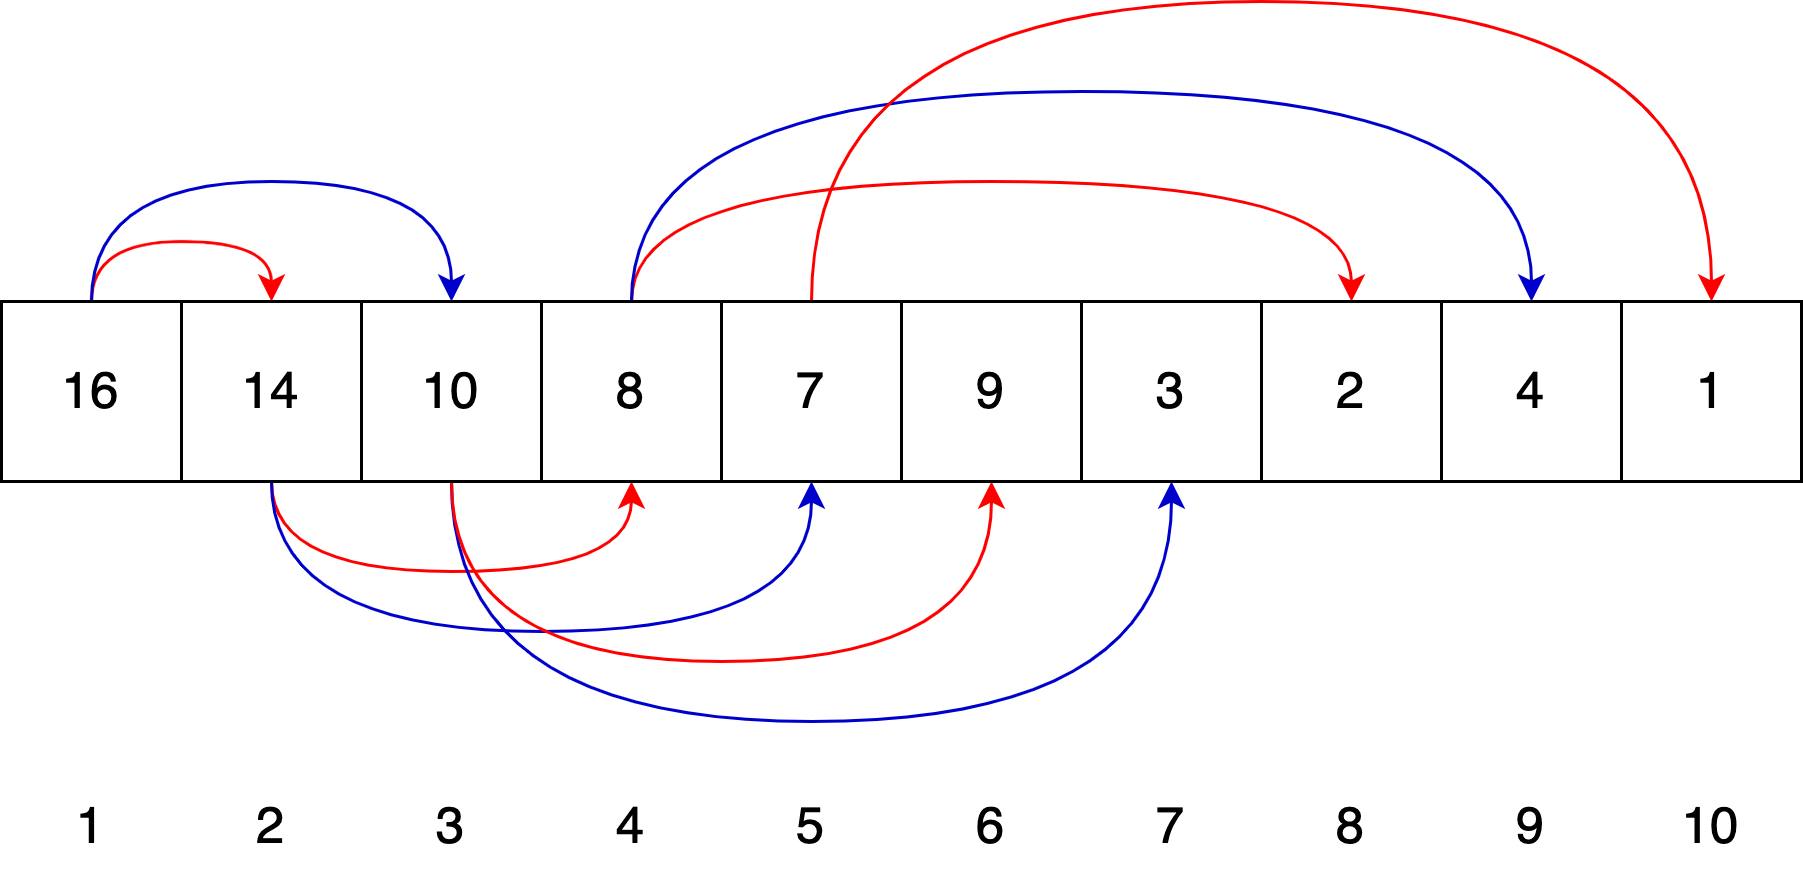
\includegraphics[scale=0.5]{img/binary-tree-in-array}
 \caption{Map between a complete binary tree and an array.} \label{fig:tree-array-map}
\end{figure}

\be
\begin{cases}
parent(i) & = \lfloor \dfrac{i}{2} \rfloor \\
left(i)   & = 2i \\
right(i)  & = 2i + 1 \\
\end{cases}
\ee

\subsection{Heapify}
\index{Binary heap!Heapify}

Heapify is the process that maintains heap property, keeping the minimum element on the top. For binary heap, we obtain a stronger property as the binary tree is recursive: every sub-tree stores its minimum element in the root. In other words, every sub-tree is also a binary heap. For the cell indexed $i$ in array representation, we examine whether all the sub-tree elements are greater than or equal to it ($\geq$), exchange when do not satisfy.

\begin{algorithmic}[1]
\Function{Heapify}{$A, i$}
  \State $n \gets |A|$
  \Loop
    \State $s \gets i$ \Comment{$s$ is the smallest}
    \State $l \gets$ \Call{Left}{$i$}, $r \gets$ \Call{Right}{$i$}
    \If{$l \leq n$ and $A[l] < A[i]$}
      \State $s \gets l$
    \EndIf
    \If{$r \leq n$ and $A[r] < A[s]$}
      \State $s \gets r$
    \EndIf
    \If{$s \neq i$}
      \State \textproc{Exchange} $A[i] \leftrightarrow A[s]$
      \State $i \gets s$
    \Else
      \State \Return
    \EndIf
  \EndLoop
\EndFunction
\end{algorithmic}

Because we recursive check sub-trees, the process time is proportion to the height of the tree. \textproc{Heapify} is bound to $O(\lg n)$, where $n$ is the length of the array. \Cref{fig:heapify} gives the steps when apply \textproc{Heapify} from $2$ to array [1, 13, 7, 3, 10, 12, 14, 15, 9, 16]. The result is [1, 3, 7, 9, 10, 12, 14, 15, 13, 16].

\begin{figure}[htbp]
  \centering
  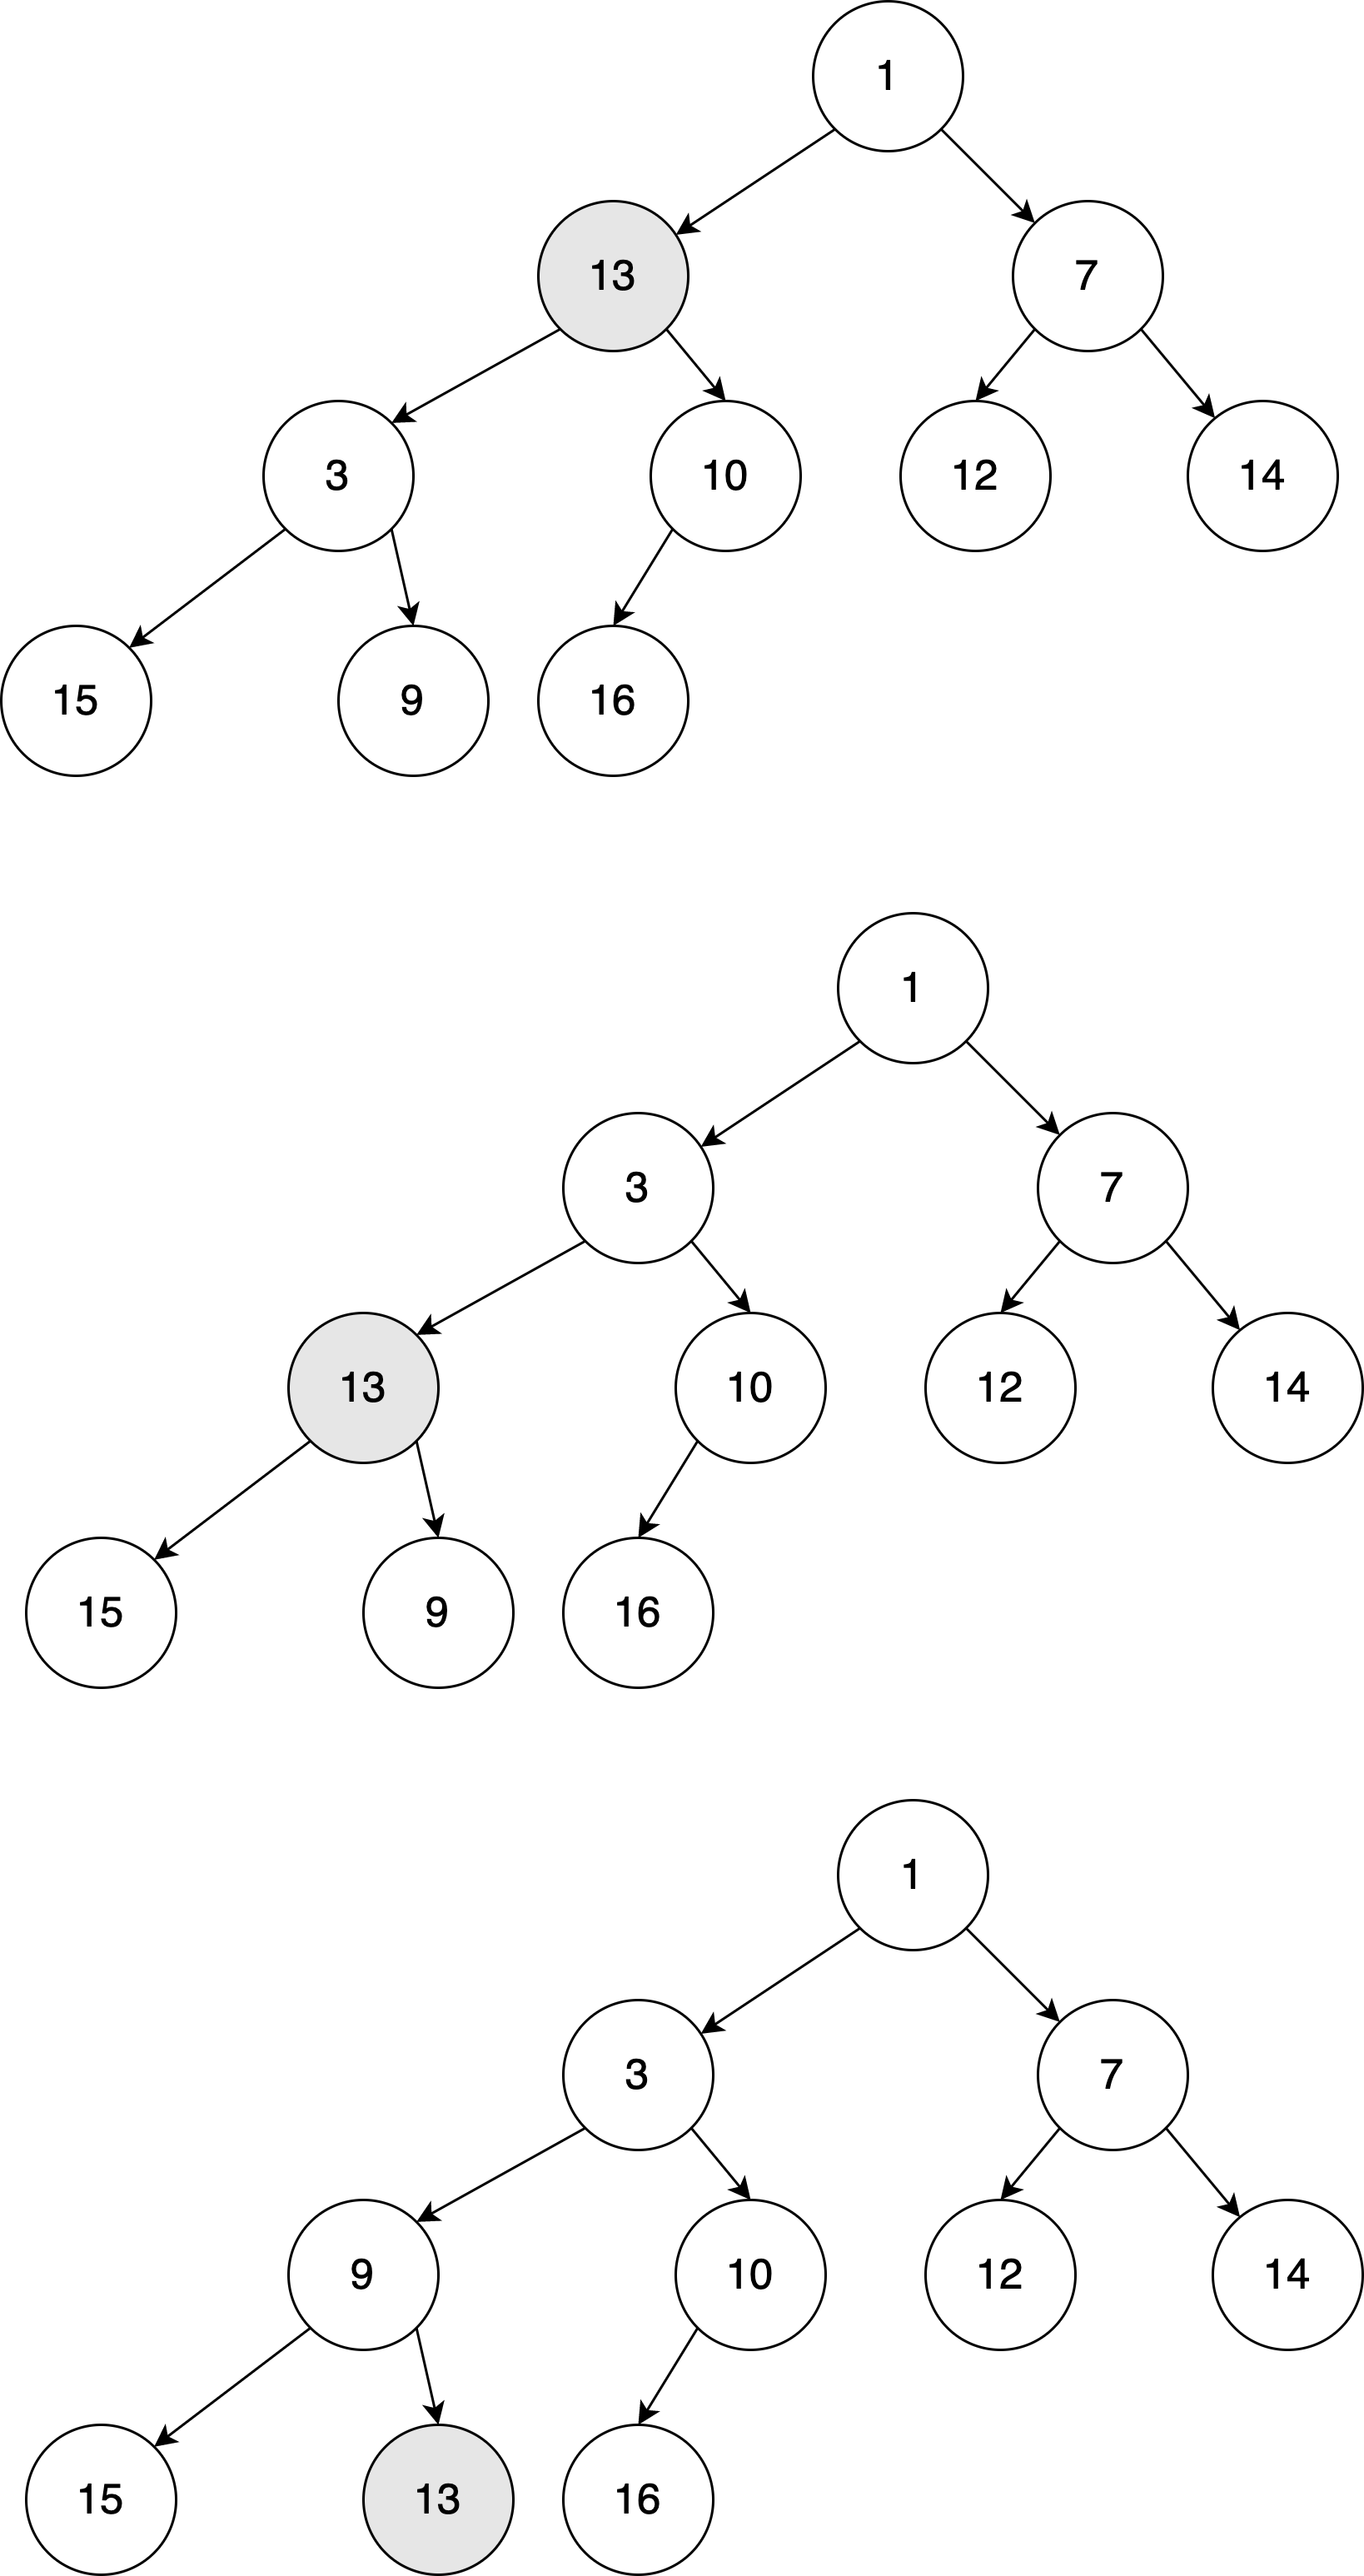
\includegraphics[scale=0.4]{img/heapify}
  \caption{Heapify. Step 1: the minimum of 13, 3, 10 is 3, exchange 3 $\leftrightarrow$ 13; Step 2: the minimum of 13, 15, 9 is 9, exchange 13 $\leftrightarrow$ 9; Step 3: 13 is leaf, terminate.}
  \label{fig:heapify}
\end{figure}

\subsection{Build}
\index{Binary heap!build}

We can build heap from an array with \textproc{Heapify}. List the numberf of nodes in each level of a complete binary tree: $1, 2, 4, 8, ...$. They are all powers of 2 except for the last level, because the tree is not necessarily full. There are at most $2^{p-1}$ nodes, where $p$ is the smallest integer satisfying $2^p - 1 \geq n$, and $n$ is the length of the array. Skip all leaves because \textproc{Heapify} takes no effect on them, we start applying \textproc{Heapify} to the last branch node (indexed at $\leq \lfloor n/2 \rfloor$) bottom-up. The build function is defined as below:

\begin{algorithmic}[1]
\Function{Build-Heap}{$A$}
  \State $n \gets |A|$
  \For{$i \gets \lfloor n/2 \rfloor$ down to $1$}
    \State \Call{Heapify}{$A, i$}
  \EndFor
\EndFunction
\end{algorithmic}

Although \textproc{Heapify} is bound $O(\lg n)$ time, \textproc{Build-Heap} is bound to $O(n)$, but not $O(n \lg n)$. We skip all leaves, check and move down a level at most for $1/4$ nodes; check and move down two levels at most for $1/8$ nodes; check and move down three levels at most for $1/16$ nodes... the total number of comparisons and moves  is up to:

\be
S = n (\frac{1}{4} + 2 \frac{1}{8} + 3 \frac{1}{16} + ...)
\label{eq:build-heap-1}
\ee

Multiply by 2 for both sides:

\be
2S = n (\frac{1}{2} + 2 \frac{1}{4} + 3 \frac{1}{8} + ...)
\label{eq:build-heap-2}
\ee

Subtract \cref{eq:build-heap-1} from \cref{eq:build-heap-2}:

\bea*{rcll}
2S - S & = & n [\dfrac{1}{2} + (2 \dfrac{1}{4} - \dfrac{1}{4}) + (3 \dfrac{1}{8} - 2 \dfrac{1}{8}) + ...] & \text{shift by one and subtract} \\
     S & = & n [\dfrac{1}{2} + \dfrac{1}{4} + \dfrac{1}{8} + ...] & \text{geometric series} \\
       & = & n
\eea*


\Cref{fig:build-heap-3} shows the steps to build a min-heap from array $[4, 1, 3, 2, 16, 9, 10, 14, 8, 7]$. The black node is where \textproc{Heapify} is applied. The grey nodes are swapped to maintain the heap property.

\begin{figure}[htbp]
  \centering
  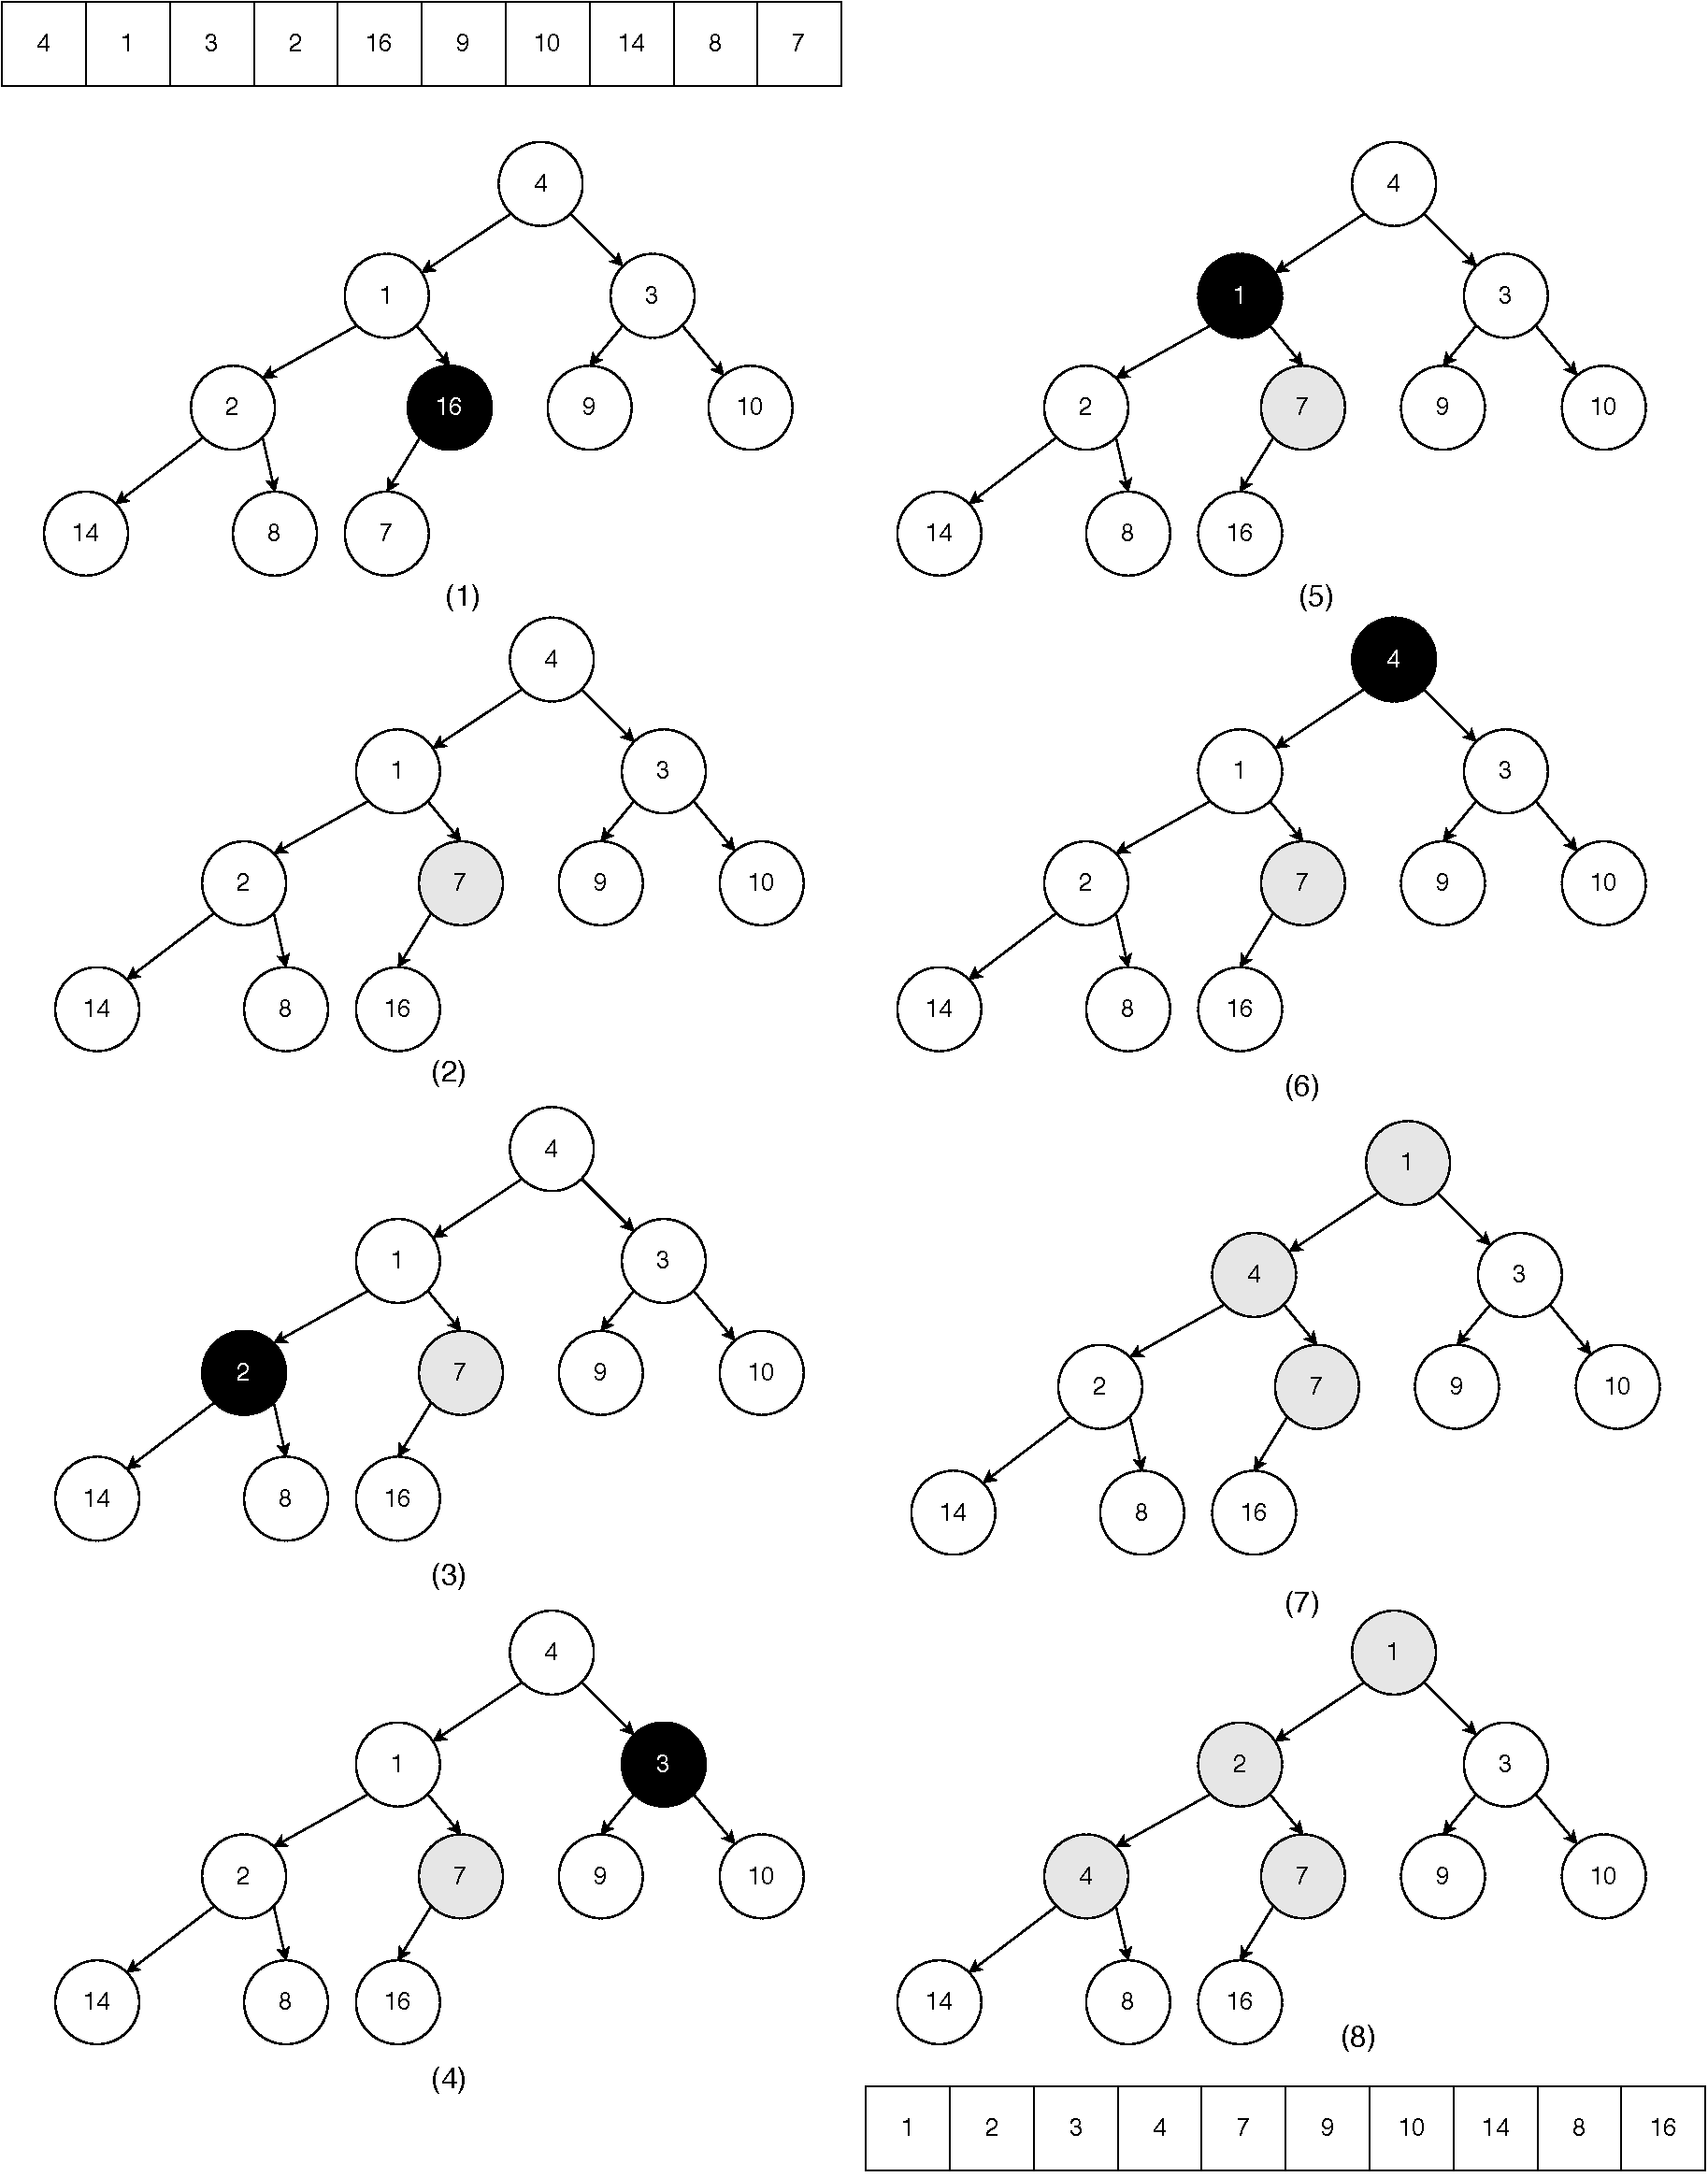
\includegraphics[scale=0.4]{img/build-heap}
  \caption{Build heap. (1) 16 > 7; (2) exchange 16 $\leftrightarrow$ 7; (3) 2 < 14 and 2 < 8; (4) 3 < 9 and 3 < 10; (5) 1 < 2 and 1 < 7; (6) 1 < 4 and 1 < 3; (7) exchange 4 $\leftrightarrow$ 1; (8) exchange 4 $\leftrightarrow$ 2, end.}
  \label{fig:build-heap-3}
\end{figure}

\subsection{Heap operations}

\index{Binary heap!top}
Heap operations include access the top, pop, lookup the top $k$ elements, decrease an element in min-heap (or increase an element in max-heap), and insert. The root of the binary heap, which is the first array cell stores the minimum: $Top(A) = A[1]$.

\index{Binary heap!pop}
After pop, the remaining elements all shift ahead a cell of the array. However, without the root, the rest is not a binary tree any more. Alternatively, we swap the head and the tail of the array, then reduce the array length by one. It's equivalent to remove a leaf but not the root. We then apply \textproc{Heapify} to the root to recover the heap property:

\begin{algorithmic}[1]
\Function{Pop}{$A$}
  \State $x \gets A [1], n \gets |A|$
  \State \textproc{Exchange} $A[1] \leftrightarrow A[n]$
  \State \Call{Remove}{$A, n$}
  \If{$A$ is not empty}
    \State \Call{Heapify}{$A$, 1}
  \EndIf
  \State \Return $x$
\EndFunction
\end{algorithmic}

\index{Binary heap!top-k}
It takes constant time to remove the last element from array, pop is bound to $O(\lg n)$ time as it calls \textproc{Heapify}. We can develop a solution to find the top $k$ elements from an array. First build a heap from the array, then repeatedly pop $k$ times:

\begin{algorithmic}[1]
\Function{Top-k}{$A, k$}
  \State $R \gets [\ ]$
  \State \Call{Build-Heap}{$A$}
  \Loop \ \textproc{Min}(k, |$A$|) times \Comment{cut off when $k > |A|$}
    \State \textproc{Append}($R$, \Call{Pop}{$A$})
  \EndLoop
  \State \Return $R$
\EndFunction
\end{algorithmic}

\index{Binary heap!decrease key}
Further, we can implement a {\em priority queue} to schedule tasks with priorities. Every time, we peek the highest priority task to run. To run an urgent task earlier, we can increase its priority, meaning to decrease an element in a min-heap, as shown in \cref{fig:decrease-key-2}.

\begin{figure}[htbp]
  \centering
  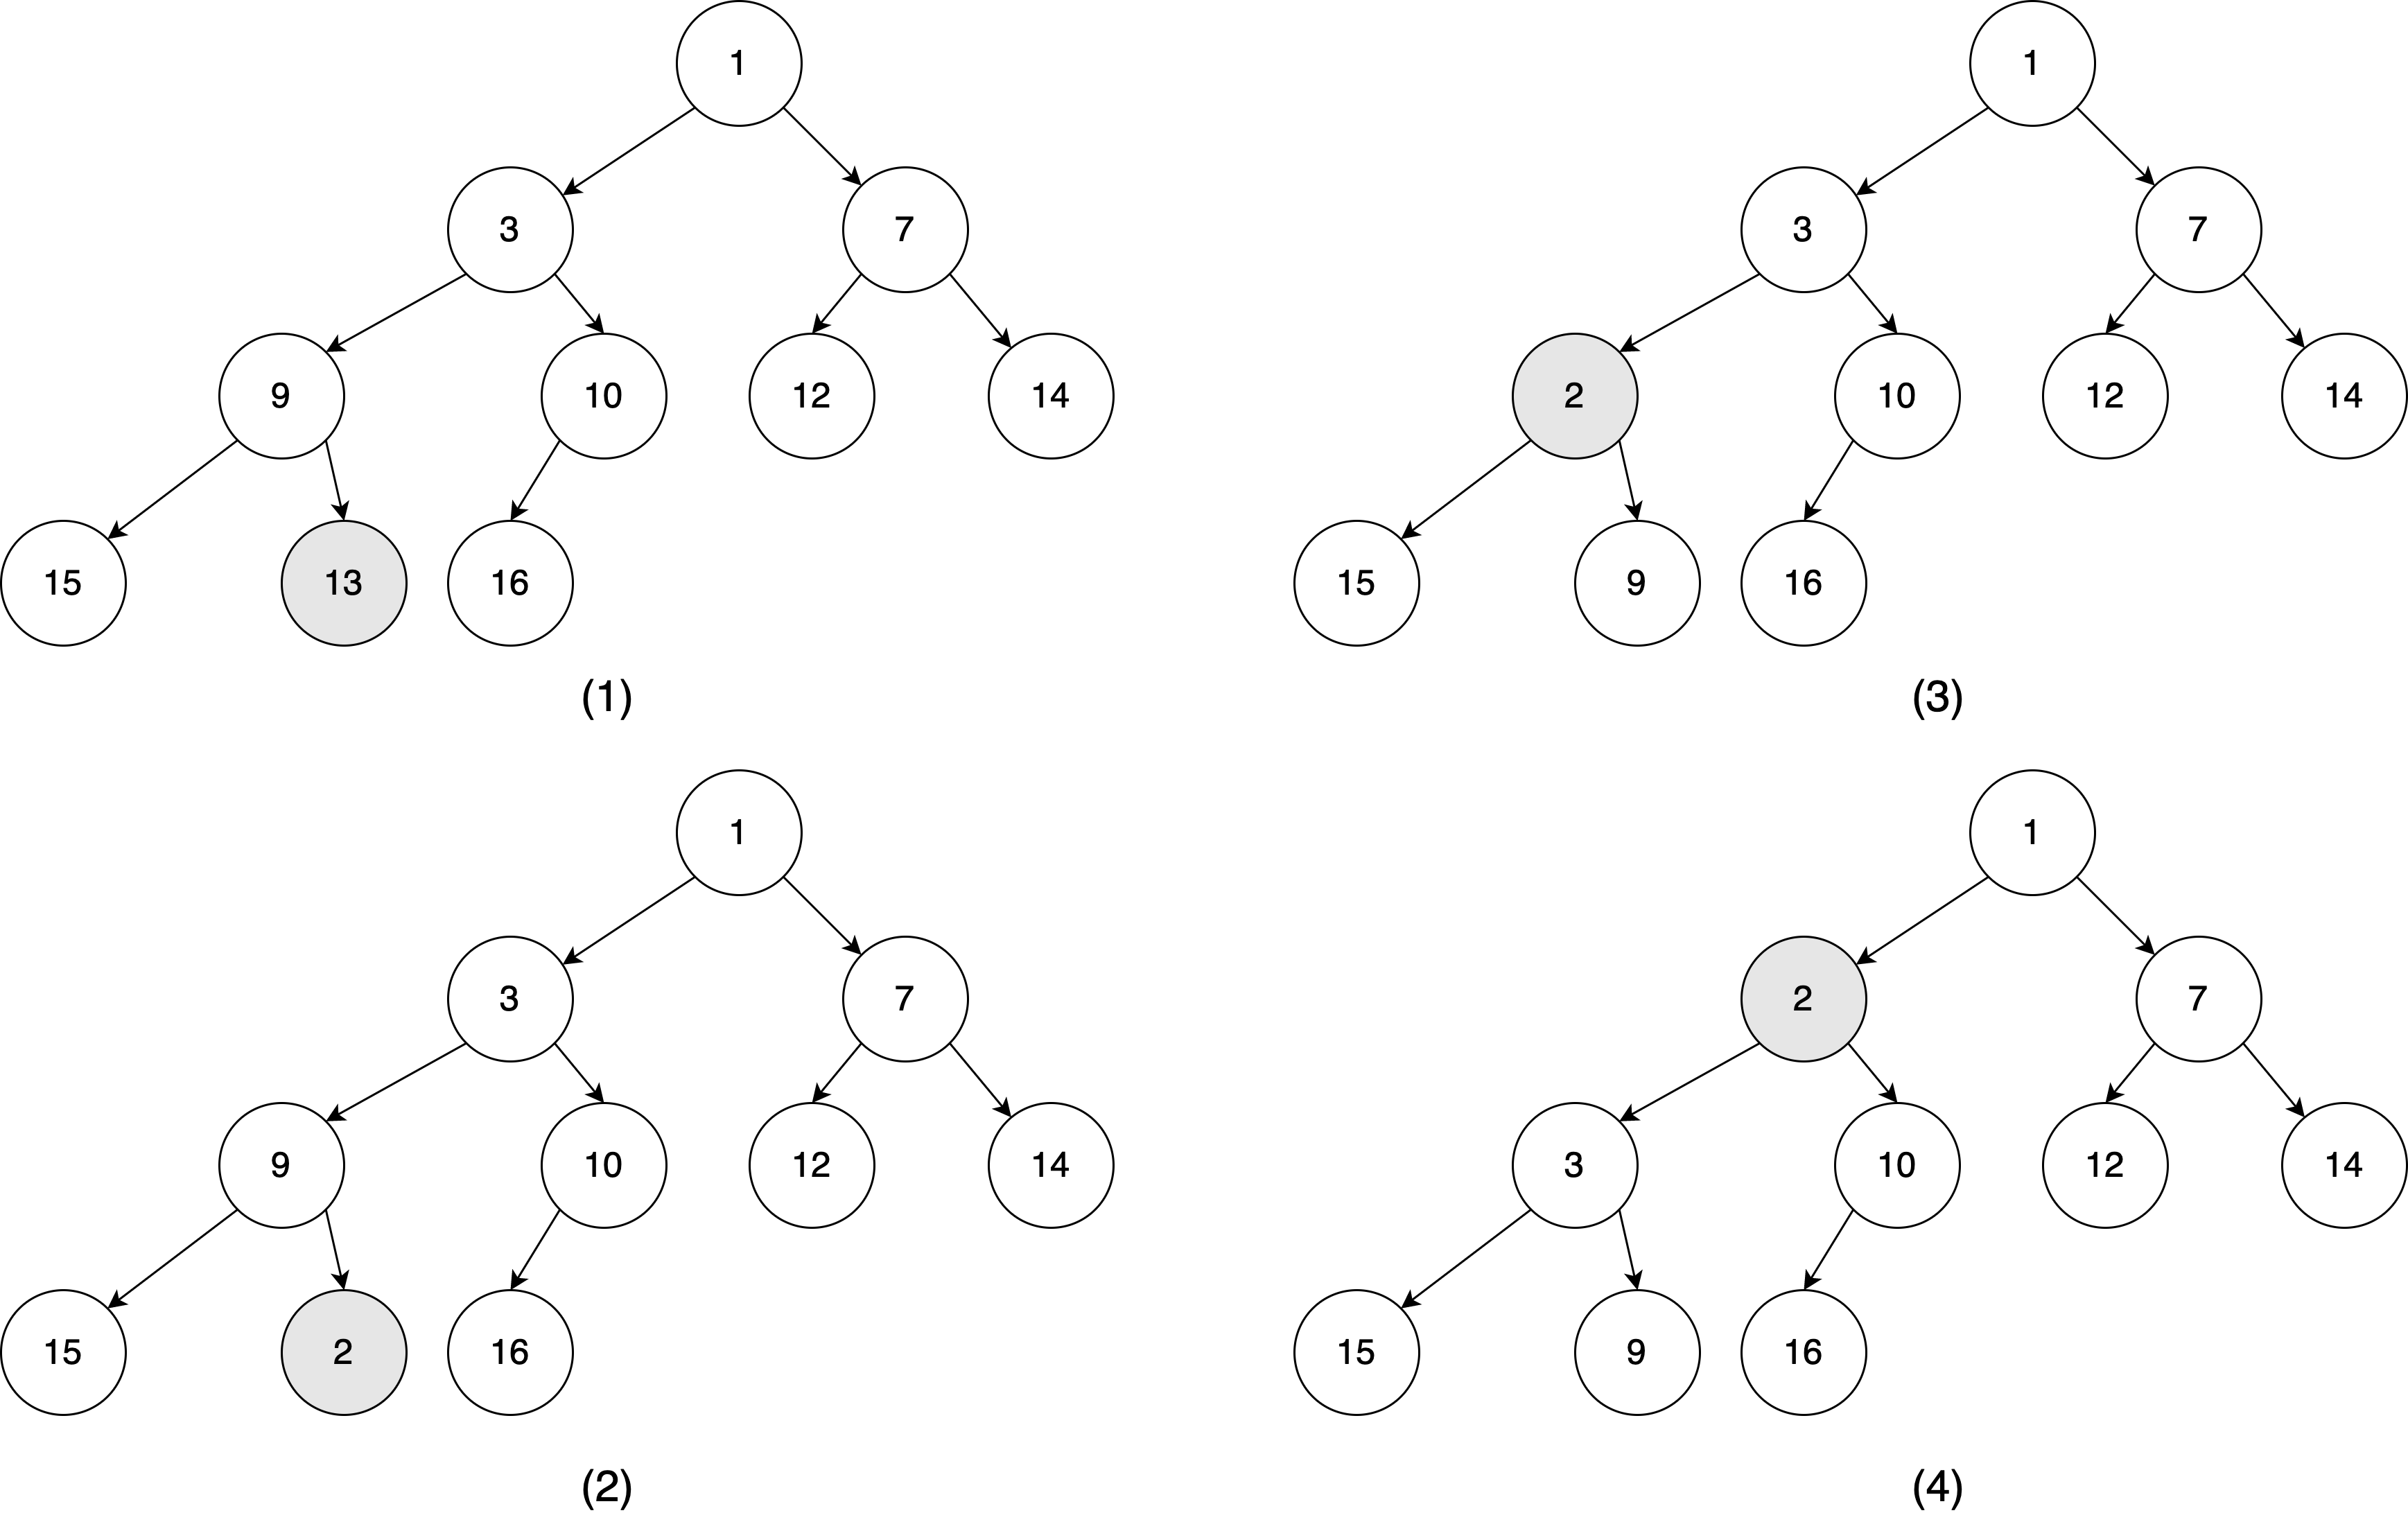
\includegraphics[scale=0.4]{img/decrease-key}
  \caption{Decrease 13 to 2. Exchange 2 and 9, then exchange with 3.}
  \label{fig:decrease-key-2}
\end{figure}

The heap property may be broken when decrease some element in a min-heap. Let the decreased element be $A[i]$, below function resumes the heap property bottom-up. It is bound to $O(\lg n)$ time.

\begin{algorithmic}[1]
\Function{Heap-Fix}{$A, i$}
  \While{$i>1$ and $A[i] < A[$ \Call{Parent}{$i$} $]$}
    \State \textproc{Exchange} $A[i] \leftrightarrow A[$ \Call{Parent}{$i$} $]$
    \State $i \gets$  \Call{Parent}{$i$}
  \EndWhile
\EndFunction
\end{algorithmic}

\index{Binary heap!insertion} \index{Binary heap!push}

We can realize push with \textproc{Heap-Fix} \cite{CLRS}. Append the new element $k$ to the tail, then apply \textproc{Heap-Fix} to recover the heap property:

\begin{algorithmic}[1]
\Function{Push}{$A, k$}
  \State \Call{Append}{$A, k$}
  \State \Call{Heap-Fix}{$A, |A|$}
\EndFunction
\end{algorithmic}

\subsection{Heap sort}
\label{heap-sort} \index{Heap sort}

We can sort elements with heap. Build a min-heap from $n$ elements (with $(n)$ time), then repeatedly pop the top to build the ascending result. Each pop is bound to $O(\lg n)$ time, the total time is bound to $O(n \lg n)$. Besides, we need another list of length $n$ to hold the result.

\begin{algorithmic}[1]
\Function{Heap-Sort}{$A$}
  \State $R \gets [\ ]$
  \State \Call{Build-Heap}{$A$}
  \While{$A \neq [\ ]$}
    \State \textproc{Append}($R$, \Call{Pop}{$A$})
  \EndWhile
  \State \Return $R$
\EndFunction
\end{algorithmic}

Robert W. Floyd developed a fast implementation with max-heap. Every time, swap the head and the tail of the array. The maximum is swapped to the expected position, the tail; and the previous tail becomes the new top. Next decrease the heap size by one, and apply \textproc{Heapify} to restore the heap property. Repeat this till the heap size decrease to one. This algorithm needn't the additional space.

\begin{algorithmic}[1]
\Function{Heap-Sort}{$A$}
  \State \Call{Build-Max-Heap}{$A$}
  \State $n \gets |A|$
  \While{$n > 1$}
    \State \textproc{Exchange} $A[1] \leftrightarrow A[n]$
    \State $n \gets n - 1$
    \State \Call{Heapify}{$A[1...n], 1$}
  \EndWhile
\EndFunction
\end{algorithmic}

\begin{Exercise}\label{ex:arrayed-binary-heap}
\Question{Consider another idea about in-place heap sort: Build a min-heap from the array $A$, the first element $a_1$ is in the right position. Treat the rest $[a_2, a_3, ..., a_n]$ as the new heap, and apply \textproc{Heapify} from $a_2$. Repeat this till the last element. Is this method correct?
\begin{algorithmic}[1]
\Function{Heap-Sort}{$A$}
  \State \Call{Build-Heap}{$A$}
  \For{$i = 1$ to $n - 1$}
    \State \Call{Heapify}{$A[i ... n], 1$}
  \EndFor
\EndFunction
\end{algorithmic}
}

\Question{Similarly, can we apply \textproc{Heapify} $k$ times from left to right to get the top-$k$ elements?
\begin{algorithmic}[1]
\Function{Top-K}{$A, k$}
  \State \Call{Build-Heap}{$A$}
  \State $n \gets |A|$
  \For {$i \gets 1$ to $min(k, n)$}
    \State \Call{Heapify}{$A[i ... n], 1$}
  \EndFor
\EndFunction
\end{algorithmic}
}
\end{Exercise}

\begin{Answer}[ref = {ex:arrayed-binary-heap}]
\Question{No, it is not correct. The sub-array $[a_2, a_3, ..., a_n]$ can't map back to binary heap. It's insufficient to only apply \textproc{Heapify} from $a_2$, we need run \textproc{Build-Heap} to rebuild the heap.}

\Question{For the same reason, it does not work.}
\end{Answer}

\section{Leftist heap and skew heap}
\label{ebheap}

With an explicit binary tree, after pop the root, there remain two sub-trees. Both are heaps as shown in \cref{fig:lvr}. How can we merge them to a new heap? To maintain the heap property, the new root must be the minimum of the remaining. We can give the two edge cases easily:

\begin{figure}[htbp]
  \centering
  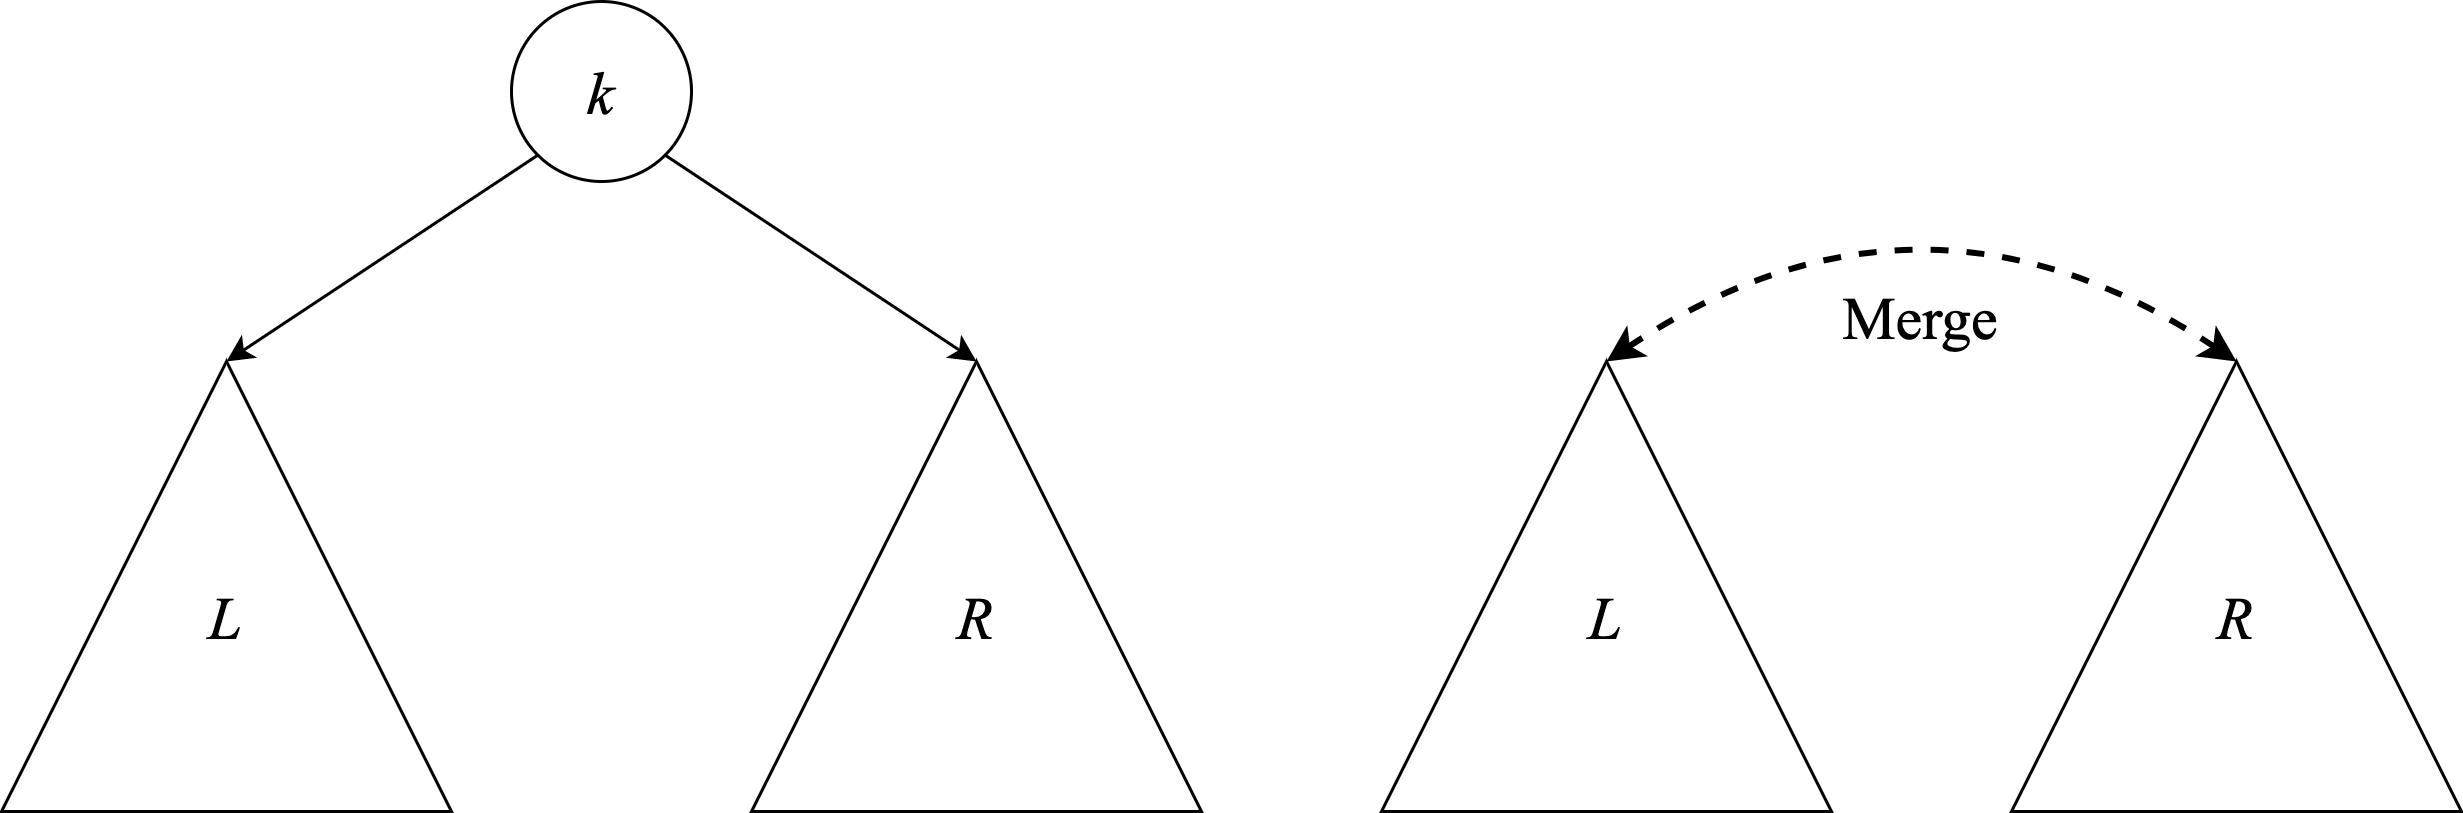
\includegraphics[scale=0.5]{img/lkr}
  \caption{Merge left and right sub-trees after pop.}
  \label{fig:lvr}
\end{figure}

\[
\begin{array}{rcl}
merge\ \nil\ R & = & R \\
merge\ L\ \nil & = & L \\
merge\ L\ R & = & ? \\
\end{array}
\]

Both left and right sub-trees are heaps. If neither is empty, each root stores the minimum respectively. We compare the two roots, and peek the smaller one as the new root. Let $L = (A, x, B)$, $R = (A', y, B')$, where $A$, $A'$, $B$, $B'$ are sub-trees. If $x < y$, then $x$ is the new root. We keep $A$, and merge $B$ and $R$ recursively; alternatively, we can keep $B$, and merge $A$ and $R$. The new heap can be $(merge(A, R), x, B)$ or $(A, x, merge(B, R))$. We always merge the right sub-tree for simplicity. This method generates the {\em leftist heap}.

\subsection{Leftist heap}
\index{Leftist heap} \index{Leftist heap!rank} \index{Leftist heap!S-value}

The leftist heap is implemented with leftist tree. C. A. Crane in 1972\cite{wiki-leftist-tree} developed the leftist tree. He defines a rank for every node (also known as $S$-value) as the distance to the nearest NIL. The rank of NIL is 0. As shown in \cref{fig:rank}, The nearest leaf node to 4 is 8, the rank of 4 is 2; Both 6 and 8 are leaves, their ranks are 1. Although the left sub-tree of 5 is not empty, its right sub-tree is NIL, hence the rank is 1. Define the merge method with rank as below. Denote the rank of the left and right sub-trees be $r_l$, $r_r$ respectively:

\begin{figure}[htbp]
  \centering
  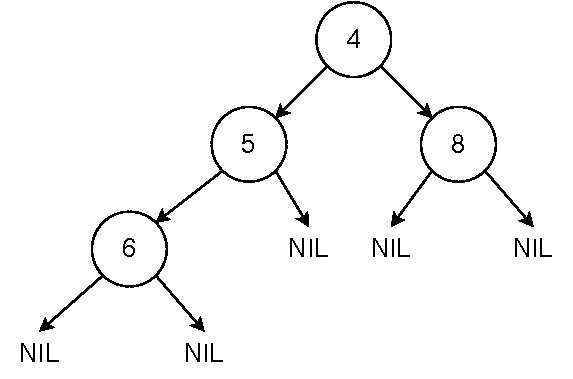
\includegraphics[scale=0.6]{img/rank}
  \caption{$rank(4) = 2$, $rank(6) = rank(8) = rank(5) = 1$.}
  \label{fig:rank}
\end{figure}

\begin{enumerate}
\item Always merge the right sub-tree;
\item When $r_l < r_r$, swap the left and right sub-trees.
\end{enumerate}

We call this merge method the `leftist property'. Basically, a leftist tree always has the shortest path to some NIL on the right. Although it seems unbalanced, there is critical fact:

\begin{theorem}
For a leftist tree $T$ of $n$ nodes, the path from the root to the rightmost NIL has at most $\lfloor \log (n + 1) \rfloor$ nodes.
\end{theorem}

We skip the proof \cite{brono-book} \cite{TAOCP}. This theorem ensures any algorithm processes along this path is bound to $O(\lg n)$ time. We define the leftist tree as a binary tree plus an additional rank. Let the none empty leftist tree be $(r, L, k, R)$:

\lstset{frame = single}
\begin{Haskell}
data LHeap a = Empty | Node Int (LHeap a) a (LHeap a)
\end{Haskell}

Function $rank$ returns the rank value:

\be
\begin{array}{rcl}
rank\ \nil & = & 0 \\
rank\ (r, L, k, R) & = & r \\
\end{array}
\ee

\index{Leftist heap!merge}
Define an auxiliary $make$ function. It compares the ranks of the sub-trees and swap them if necessary.

\be
make(A, k, B) = \begin{cases}
  rank(A) < rank(B) : & (1 + rank(A), B, k, A) \\
  \text{otherwise}: & (1 + rank(B), A, k, B) \\
  \end{cases}
\ee

For the two trees $A$ and $B$, if $rank(A)$ is smaller, set $B$ as the left sub-tree, and $A$ as the right. The rank of the new node is $1 + rank(A)$; otherwise if $rank(B)$ is smaller, set $A$ as the left sub-tree, and $B$ as the right. The rank of the new node is $1 + rank(B)$. Given two leftist heaps, and denote them as $H_1 = (r_1, L_1, K_1, R_1)$ and $H_2 = (r_2, L_2, k_2, R_2)$ if not empty, define merge:

\be
\begin{array}{rcl}
  \textit{merge}\ \nil\ H_2 & = & H_2 \\
  \textit{merge}\ H_1\ \nil & = & H_1 \\
  \textit{merge}\ H_1\ H_2 & = & \begin{cases}
  k_1 < k_2 : & make(L_1, k_1, \textit{merge}\ R_1\ H_2)  \\
  \text{otherwise}: & make(L_2, k_2, \textit{merge}\ H_1\ R_2) \\
  \end{cases}
\end{array}
\ee

We always $merge$ to the right sub-tree recursively to maintain the leftist property. It is bound to $O(\lg n)$ time. The binary heap implemented with array performs well in most cases, suitable for the modern cache technology. However, it takes $O(n)$ time to merge, because it needs concatenate two arrays, and rebuild the heap\cite{NIST}:

\begin{algorithmic}[1]
\Function{Merge-Heap}{$A, B$}
  \State $C \gets$ \Call{Concat}{$A, B$}
  \State \Call{Build-Heap}{$C$}
\EndFunction
\end{algorithmic}

\index{Leftist heap!top} \index{Leftist heap!pop}

We can access the top of the leftist heap in constant time(assume it is not empty):

\be
top\ (r, L, k, R) = k
\ee

After pop the root, we merge the two sub-trees in $O(\lg n)$ time.

\be
pop\ (r, L, k, R) = merge\ L\ R
\ee

\index{Leftist heap!insert}
To insert a new element $k$, create a leaf of $k$, then merge it to the heap:

\be
insert\ k\ H = merge\ (1, \nil, k, \nil)\ H
\ee

\index{Leftist heap!heap sort}
We can build a leftist heap from a list as (Curried form): $build = fold_r\ insert\ \nil$. Then repeatedly pop the minimum to output the sorted result:

\begin{figure}[htbp]
  \centering
  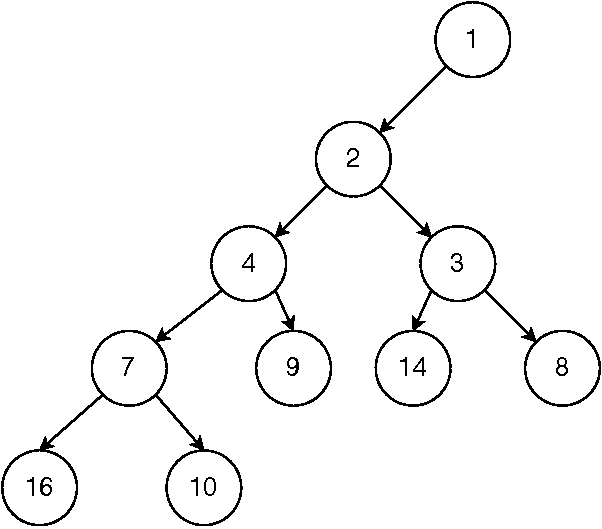
\includegraphics[scale=0.5]{img/leftist-tree}
  \caption{Build the leftist heap from $[9, 4, 16, 7, 10, 2, 14, 3, 8, 1]$.}
  \label{fig:leftist-tree}
\end{figure}

\be
sort = heapSort \circ build
\ee

Where

\be
\begin{array}{rcl}
heapSort\ \nil & = & [\ ] \\
heapSort\ H & = & (top\ H) : (heapSort\ (pop\ H)) \\
\end{array}
\ee

It pops $n$ times, each takes $O(\lg n)$ time. The total time is bound to $O(n \lg n)$.

\subsection{Skew heap}
\label{skew-heap} \index{Skew heap}

Leftist heap may lead to unbalanced tree in some cases as shown in \cref{fig:unbalanced-leftist-tree}. Skew heap is a self-adjusting heap. It simplifies the leftist heap and improves balance\cite{wiki-skew-heap} \cite{self-adjusting-heaps}. To build the leftist heap, we swap the left and right sub-trees when the rank on left is smaller than the right. However, this method can't handle the case that either sub-tree has a NIL node. The rank is always 1 no matter how big the sub-tree is. Skew heap always swaps the sub-trees for simplification.

\begin{figure}[htbp]
  \centering
  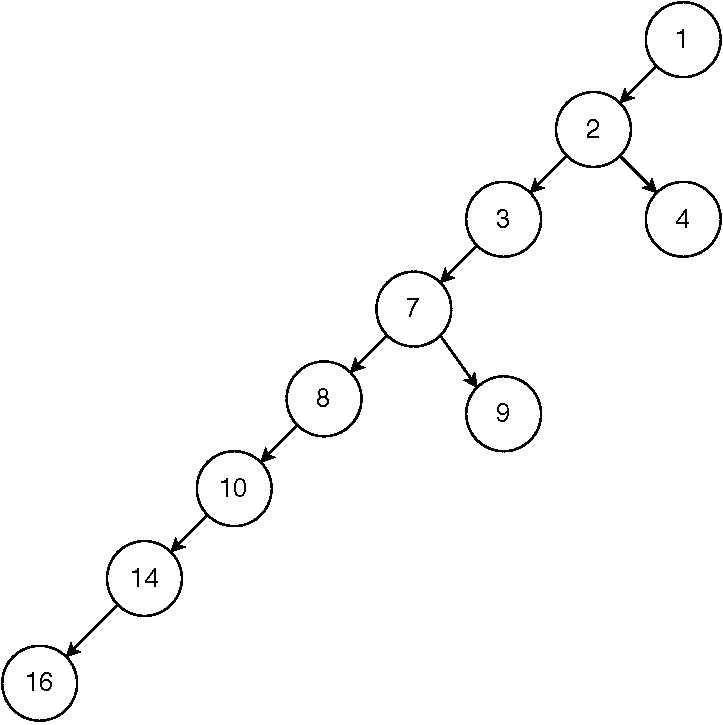
\includegraphics[scale=0.45]{img/unbalanced-leftist-tree}
  \caption{Leftist heap built from $[16, 14, 10, 8, 7, 9, 3, 2, 4, 1]$.}
  \label{fig:unbalanced-leftist-tree}
\end{figure}

Skew heap is implemented with skew tree. A skew tree is a binary tree. The root stores the minimum element, every sub-tree is also a skew tree. Skew tree needn't the rank. We can directly re-use the binary tree definition. Denote the none empty tree as $(L, k, R)$.

\begin{Haskell}
data SHeap a = Empty | Node (SHeap a) a (SHeap a)
\end{Haskell}

\index{Skew heap!merge} \index{Skew heap!insertion} \index{Skew heap!top} \index{Skew heap!pop}

When merge two none empty skew trees $H_1 = (L_1, k_1, R_1)$ and $H_2 =(L_2, k_2, R_2)$, if $k_1 < k_2$, then choose $k_1$ (otherwise $k_2$) as the new root. Then merge the greater one with a sub-tree. We can either merge $H_2$ with $L_1$, or merge $H_2$ with $R_1$. We choose $R_1$, and swap the left and right sub-trees. The result is $(\textit{merge}(R_1, H_2), k_1, L_1)$.

\be
\begin{array}{rcl}
\textit{merge}\ \nil\ H_2 & = & H_2 \\
\textit{merge}\ H_1\ \nil & = & H_1 \\
\textit{merge}\ H_1\ H_2\ & = & \begin{cases}
  k_1 < k_2: & (\textit{merge}(R_1, H_2), k_1, L_1) \\
  \text{otherwise}: & (\textit{merge}(H_1, R_2), k_2, L_2) \\
\end{cases}
\end{array}
\ee

The other operations, including insert, top, and pop are implemented with \textit{merge}. Skew heap outputs a balanced tree even for ordered list as shown in \cref{fig:skew-tree}.

\begin{figure}[htbp]
  \centering
  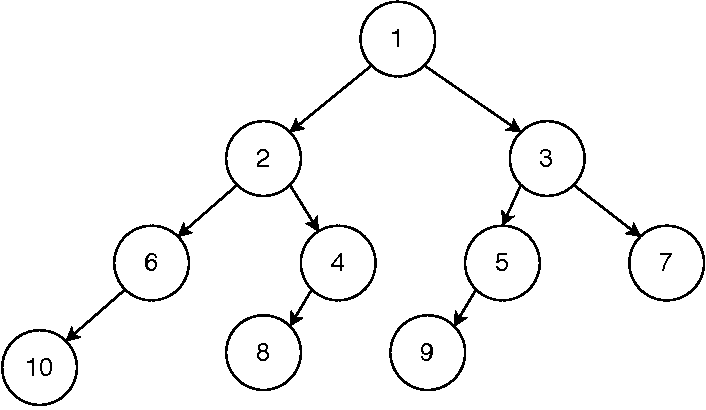
\includegraphics[scale=0.5]{img/skew-tree}
  \caption{Skew tree built from $[1, 2, ..., 10]$.}
  \label{fig:skew-tree}
\end{figure}

\section{Splay heap}
\label{splayheap} \index{Splay heap}

Both leftist heap and skew heap are implemented with binary trees. If change to binary search tree, then the minimum will not be in root. We need $O(\lg n)$ time to locate the minimum. The performance downgrades if the tree is not balanced. Although we can use the red-black tree to secure balancing, the splay tree provides a simple solution. It dynamically `splays' to balance the tree. Splay tree takes cache-like approach. It rotates the node currently being accessed to the root, reduces the access time for the next visit. We define such operation as 'splay'. The tree tends to be more balanced after multiple splays. Most splay tree operations perform in amortized $O(\lg n)$ time. Sleator and Tarjan developed splay tree in 1985\cite{wiki-splay-tree}\cite{self-adjusting-trees}.

\subsection{Splay}
\index{Splay heap!splay}

We give two implementations. The first is pattern matching, it needs match multiple cases; the second has the uniformed form, but the implementation is complex. When access node $x$, denote the parent node as $p$, and grand parent node (if there is) as $g$. There are 3 cases, each has two symmetric sub-cases. \Cref{fig:splay} shows one:

\begin{enumerate}
\item {\em Zig-zig}: Both $x$ and $p$ are on the left; or on the right. We rotate twice to make $x$ as root.

\item {\em Zig-zag}: $x$ is on the left, while $p$ is on the right; or $x$ is on the right, while $P$ is on the left. After rotation, $x$ becomes the root, $p$ and $g$ are siblings.

\item {\em Zig}: $p$ is the root, we rotate to make $x$ as root.
\end{enumerate}

\begin{figure}[htbp]
  \centering
  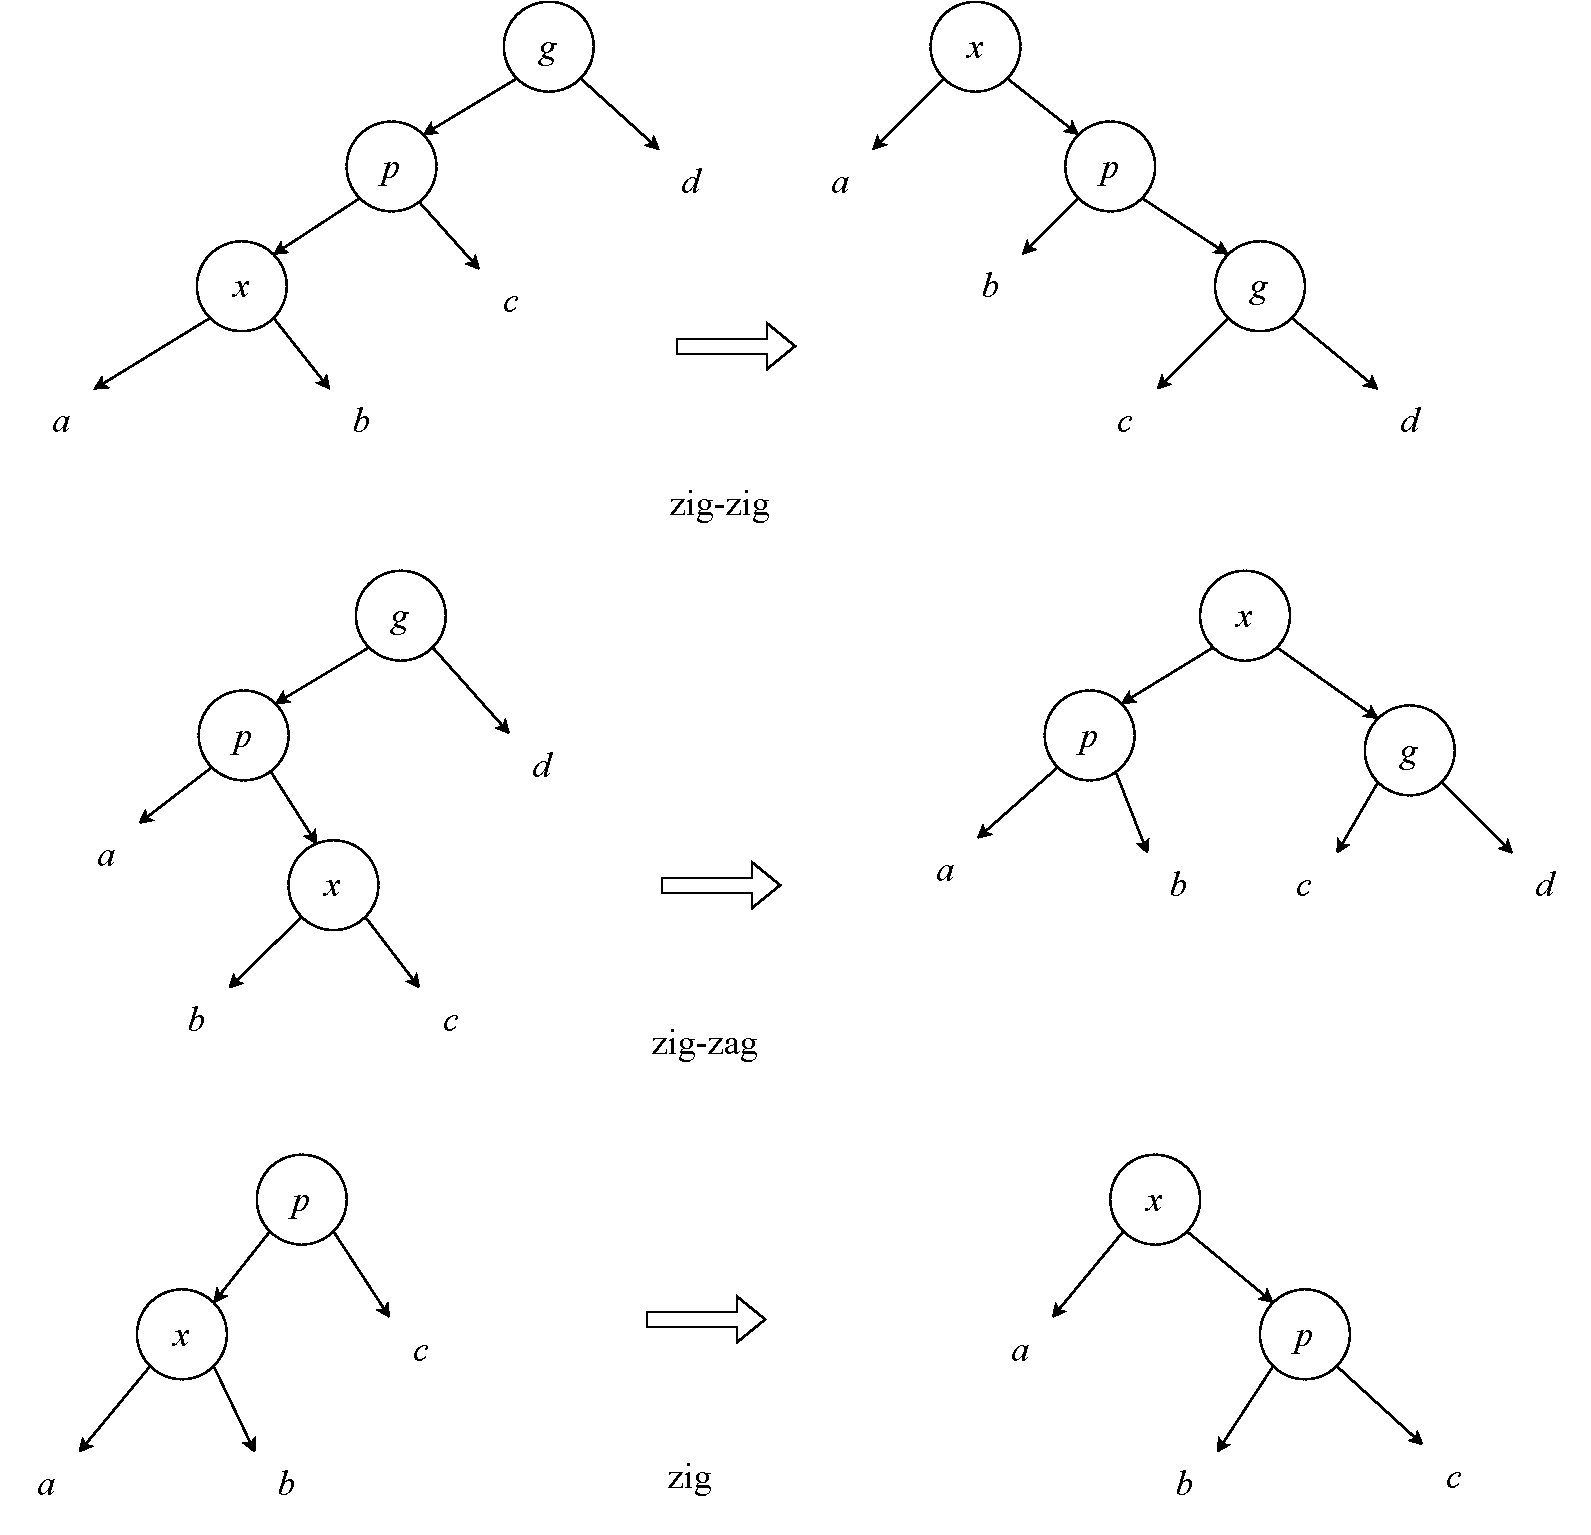
\includegraphics[scale=0.45]{img/splay}
  \caption{\textbf{zig-zig}: $x$ and $p$ are both on left or right, $x$ becomes the new root. \textbf{zig-zag}: $x$ and $p$ are on different sides, $x$ becomes the new root, $p$ and $g$ are siblings. \textbf{zig}: $p$ is the root, rotate to make $x$ as the root.}
  \label{fig:splay}
\end{figure}

There are total 6 cases. Let the none empty tree be $T=(L, k, R)$, define splay as below when access element $y$:

\be
\begin{array}{rcll}
splay\ y\ (((a, x, b), p, c), g, d) & = & \begin{cases}
    x = y: & (a, x, (b, p, (c, g, d))) \\
    \text{otherwise}: & T \\
  \end{cases} & \text{zig-zig} \\
splay\ y\ (a, g, (b, p, (c, x, d))) & = & \begin{cases}
    x = y: & (((a, g, b), p, c), x, d) \\
    \text{otherwise}: & T \\
  \end{cases} & \text{zig-zig symmetric} \\
splay\ y\ (a, p, (b, x, c), g, d) & = & \begin{cases}
    x = y: & ((a, p, b), x, (c, g, d)) \\
    \text{otherwise}: & T \\
  \end{cases} & \text{zig-zag} \\
splay\ y\ (a, g, ((b, x, c), p, d)) & = & \begin{cases}
    x = y: & ((a, g, b), x, (c, p, d)) \\
    \text{otherwise}: & T \\
  \end{cases} & \text{zig-zag symmetric} \\
splay\ y\ ((a, x, b), p, c) & = & \begin{cases}
    x = y: & (a, x, (b, p, c)) \\
    \text{otherwise}: & T \\
  \end{cases} & \text{zig} \\
splay\ y\ (a, p, (b, x, c)) & = & \begin{cases}
    x = y: & ((a, p, b), x, c) \\
    \text{otherwise}: & T \\
  \end{cases} & \text{zig symmetric} \\
splay\ y\ T & = & T & \text{others} \\
\end{array}
\ee

The tree is unchanged for all other cases. Every time when insert, we trigger splay to adjust the balance. If the tree is empty, the result is a leaf; otherwise, compare the new element and the root, then recursively insert to left (less than) or right (greater than) sub-tree and splay.

\be
\begin{array}{rcl}
insert\ y\ \nil & = & (\nil, y, \nil) \\
insert\ y\ (L, x, R) & = & \begin{cases}
  y < x: & splay\ y\ ((insert\ y\ L), x, R)  \\
  \text{otherwise}: & splay\ y\ (L, x, (insert\ y\ R)) \\
\end{cases}
\end{array}
\ee

\begin{figure}[htbp]
  \centering
  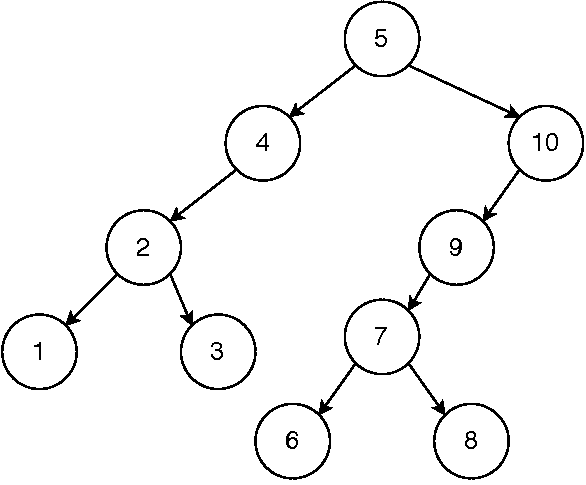
\includegraphics[scale=0.5]{img/splay-tree}
  \caption{Splay tree built from $[1, 2, ..., 10]$.}
  \label{fig:splay-result}
\end{figure}

\Cref{fig:splay-result} gives the splay tree built from $[1, 2, ..., 10]$. It generates a relative balanced tree. Okasaki gives a simple rule for splaying \cite{okasaki-book}. Whenever follow two left or two right branches continuously, rotate the two nodes. When access $x$, if have moved left or right twice, then partition $T$ as $L$ and $R$ recursively, where $L$ contains all elements less than $x$, while $R$ contains the remaining. Then create a new tree with $x$ as the root, and $L$, $R$ as the sub-trees.

\be
\resizebox{\linewidth}{!}{\ensuremath{
\begin{array}{l}
\begin{array}{rcl}
partition\ y\ \nil & = & (\nil, \nil) \\
partition\ y\ (L, x, R) & = &  \\
\end{array} \\
\quad
\begin{cases}
  x < y & \begin{cases}
      R = \nil & (T, \nil) \\
      R = (L', x', R') & \begin{cases}
          x' < y & (((L, x, L'), x', A), B) \\
                  & \text{where: }(A, B) = partition\ y\ R' \\
          \text{otherwise} & ((L, x, A), (B, x', R')) \\
                      & \text{where: }(A, B) = partition\ y\ L' \\
        \end{cases} \\
    \end{cases} \\
  \text{otherwise} & \begin{cases}
      L = \nil & (\nil, T) \\
      L = (L', x', R') & \begin{cases}
         y < x' & (A, (L', x', (R', x, R))) \\
                 & \text{where: }(A, B) = partition\ y\ L' \\
         \text{otherwise} & ((L', x', A), (B, x, R)) \\
                 & \text{where: }(A, B) = partition\ y\ R' \\
      \end{cases} \\
    \end{cases}
  \end{cases} \\
\end{array}
}}
\ee

Function $partition$ takes a pivot $y$, and a tree $T$. For empty tree, the result is $(\nil, \nil)$; otherwise for tree $(L, x, R)$, if $x < y$, there are two sub-cases: (1) $R$ is empty. All elements in the binary search tree are less then $y$, hence the result is $(T, \nil)$; (2) Let $R = (L', x', R')$, if $x' < y$, we recursively partition $R'$ with $y$. Put all elements less than $y$ in $A$, and the rest in $B$. The result is a pair of trees: $((L, x, L'), x', A)$ and $B$. If $x' > y$, then recursively partition $L'$ with $y$ to obtain $(A, B)$. The result is also a pair of $(L, x, A)$ and $(B, x', R')$. When $y < x$, the result is symmetric.

\index{Splay heap!insert}
Alternatively, we can define insert with $partition$. When insert a new element $k$ to splay heap $T$, we first partition the heap to two sub-trees of $L$ and $R$. Where $L$ contains all elements smaller than $k$, while $R$ contains the rest. Then construct a new tree with $k$ as the root, and $L$, $R$ as the sub-trees.

\be
insert\ k\ T = (L, k, R), \text{where}: (L, R) = partition\ k\ T
\ee

\subsection{Pop}
\index{Splay heap!top} \index{Splay heap!pop}

Since splay tree is essentially a binary search tree, the minimum is at the left most. We need keep traversing the left sub-tree to access the heap `top'. Let the none empty tree be $T = (L, k, R)$, we define the $top$ function as below:

\be
\begin{array}{rcl}
top\ (\nil, k, R) & = & k \\
top\ (L, k, R) & = & top\ L \\
\end{array}
\ee

This is equivalent to $min$ for the binary search tree. When pop, we need remove the minimum. We apply splay when move left twice.

\be
\begin{array}{rcl}
pop\ (\nil, k, R) & = & R \\
pop\ ((\nil, k', R'), k, R) & = & (R', k, R) \\
pop\ ((L', k', R'), k, R) & = & (pop\ L', k', (R', k, R)) \\
\end{array}
\ee

The third row performs splaying without calling $partition$. It uses the binary search tree property. Top and pop are bound to $O(\lg n)$ time when the splay tree is balanced.

\subsection{Merge}
\index{Splay heap!merge}

We can implement $merge$ with $partition$ to obtain the $O(\lg n)$ time bound. When merge two none-empty splay trees, we choose a root as the pivot to partition the other tree, then recursively merge the sub-trees:

\be
\begin{array}{rcl}
merge\ \nil\ T & = & T \\
merge\ (L, x, R)\ T & = & ((merge\ L\ L')\ x\ (merge\ R\ R')) \\
\end{array}
\ee

where

\[
  (L', R') = partition\ x\ T
\]

If a heap is empty, then the result is the other heap; otherwise, let a heap be $(L, x, R)$. We use $x$ to partition $T$ to $(L', R')$, where $L$ contains all elements less than $x$ in $T$, while $R'$ contains the rest. Then we recursively merge $L$ and $L'$ to the left sub-tree, and merge $R$ and $R'$ to the right sub-tree.

\section{Summary}

We give the generic definition of binary heap in this chapter. There are several implementations. The array based representation is suitable for imperative implementation. It maps a complete binary tree to array, supports random access any element. We also directly use the binary tree to implement the heap in functional way. Most operations are bound to $O(\lg n)$ time, some are $O(1)$ amortized time. Okasaki gave detailed analysis\cite{okasaki-book}. When extend from binary tree to $k$-ary tree, we obtain binomial heap, Fibonacci heap, and pairing heap. We introduce these heaps in chapter 10.

\begin{Exercise}\label{ex:other-binary-heaps}
\Question{Realize leftist heap and skew heap in imperative approach.} % exclude splay heap
\Question{Define fold for heap.}
\end{Exercise}

\begin{Answer}[ref = {ex:other-binary-heaps}]
\Question{Realize leftist heap and skew heap in imperative approach.

We add a parent reference in the node definition for easy back-tracking.

\begin{Bourbaki}
data Node<T> {
    T value
    Int rank = 1
    Node<T> left = null
    Node<T> right = null
    Node<T> parent = null
}
\end{Bourbaki}

When merge two leftist heaps, we firstly top-down merge along the right sub-tree, then bottom-up update the rank along the parent reference, swap the sub-trees if the left has the smaller rank. To simplify the empty tree handling, we use a sentinel node.

\begin{Bourbaki}
Node<T> merge(Node<T> a, Node<T> b) {
    var h = Node(null)  // the sentinel node
    while a != null and b != null {
        if b.value < a.value then swap(a, b)
        var c = Node(a.value, parent = h, left = a.left)
        h.right = c
        h = c
        a = a.right
    }
    h.right = if a != null then a else b
    while h.parent != null {
        if rank(h.left) < rank(h.right) then swap(h.left, h.right)
        h.rank = 1 + rank(h.right)
        h = h.parent
    }
    h = h.right
    if h != null then h.parent = null
    return h
}

Int rank(Node<T> x) = if x != null then x.rank else 0

Node<T> insert(Node<T> h, T x) = merge(Node(x), h)

T top(Node<T> h) = h.value

Node<T> pop(Node<T> h) = merge(h.left, h.right)
\end{Bourbaki}

The skew heap is more simple. We needn't update the rank, nor need the parent and back-track.

\begin{Bourbaki}
data Node<T> {
    T value
    Node<T> left = null
    Node<T> right = null
}
\end{Bourbaki}

Below is the merge function, the others are same as the leftist heap.
\begin{Bourbaki}
Node<T> merge(Node<T> a, Node<T> b) {
    var h = Node(None)
    var root = h
    while a != null and b != null {
        if b.value < a.value then swap(a, b)
        var c = Node(a.value, left = null, right = a.left)
        h.left = c
        h = c
        a = a.right
    }
    h.left = if a != null then a else b
    root = root.left
    return root
}
\end{Bourbaki}
}
\Question{Define fold for heap.

\[
\begin{array}{rcl}
fold\ f\ z\ \nil & = & z \\
fold\ f\ z\ H & = & fold\ f\ (f\ (top\ H)\ z)\ (pop\ H) \\
\end{array}
\]
}
\end{Answer}

\section{Appendix - example programs}

For the complete binary tree represented by array, access parent, and sub-trees with bit-wise operation (index from 0):

\begin{lstlisting}[language = Bourbaki]
Int parent(Int i) = ((i + 1) >> 1) - 1

Int left(Int i) = (i << 1) + 1

Int right(Int i) = (i + 1) << 1
\end{lstlisting}

Heapify, parameterized the comparison:

\begin{lstlisting}[language = Bourbaki]
void heapify([K] a, Int i, Less<K> lt) {
    Int l, r, m
    Int n = length(a)
    loop {
        m = i
        l = left(i)
        r = right(i)
        if l < n and lt(a[l], a[i]) then m = l
        if r < n and lt(a[r], a[m]) then m = r
        if m != i {
            swap(a, i, m);
            i = m
        } else {
            break
        }
    }
}
\end{lstlisting}

Build the binary heap from array:

\begin{lstlisting}[language = Bourbaki]
void buildHeap([K] a, Less<K> lt) {
    Int n = length(a)
    for Int i = (n-1) / 2 downto 0 {
        heapify(a, i, lt)
    }
}
\end{lstlisting}

Pop:

\begin{lstlisting}[language = Bourbaki]
K pop([K] a, Less<K> lt) {
    var n = length(a)
    t = a[n]
    swap(a, 0, n - 1)
    remove(a, n - 1)
    if a != [] then heapify(a, 0, lt)
    return t
}
\end{lstlisting}

Obtain the top-$k$ elements:

\begin{lstlisting}[language = Bourbaki]
[K] topk([K] a, Int k, Less<K> lt) {
    buildHeap(a, lt)
    [K] r = []
    loop min(k, length(a)) {
        append(r, pop(a, lt))
    }
    return r
}
\end{lstlisting}

Decrease the key in min-heap:

\begin{lstlisting}[language = Bourbaki]
void decreaseKey([K] a, Int i, K k, Less<K> lt) {
    if lt(k, a[i]) {
        a[i] = k
        heapFix(a, i, lt)
    }
}

void heapFix([K] a, Int i, Less<K> lt) {
    while i > 0 and lt(a[i], a[parent(i)]) {
        swap(a, i, parent(i))
        i = parent(i)
    }
}
\end{lstlisting}

Push new element:

\begin{lstlisting}[language = Bourbaki]
void push([K] a, K k, less<K> lt) {
    append(a, k)
    heapFix(a, length(a) - 1, lt)
}
\end{lstlisting}

Heap sort:

\begin{lstlisting}[language = Bourbaki]
void heapSort([K] a, less<K> lt) {
    buildHeap(a, not . lt)
    n = length(a)
    while n > 1 {
        swap(a, 0, n - 1)
        n = n - 1
        heapify(a[0 .. (n - 1)], 0, not . lt)
    }
}
\end{lstlisting}

Merge two leftist heaps:

\begin{Haskell}
merge E h = h
merge h E = h
merge h1@(Node _ x l r) h2@(Node _ y l' r') =
    if x < y then makeNode x l (merge r h2)
    else makeNode y l' (merge h1 r')

makeNode x a b = if rank a < rank b then Node (rank a + 1) x b a
                 else Node (rank b + 1) x a b
\end{Haskell}

Merge two skew heaps:

\begin{Haskell}
merge E h = h
merge h E = h
merge h1@(Node x l r) h2@(Node y l' r') =
    if x < y then Node x (merge r h2) l
    else Node y (merge h1 r') l'
\end{Haskell}

Splay operation:

\begin{Haskell}
-- zig-zig
splay t@(Node (Node (Node a x b) p c) g d) y =
    if x == y then Node a x (Node b p (Node c g d)) else t
splay t@(Node a g (Node b p (Node c x d))) y =
    if x == y then Node (Node (Node a g b) p c) x d else t
-- zig-zag
splay t@(Node (Node a p (Node b x c)) g d) y =
    if x == y then Node (Node a p b) x (Node c g d) else t
splay t@(Node a g (Node (Node b x c) p d)) y =
    if x == y then Node (Node a g b) x (Node c p d) else t
-- zig
splay t@(Node (Node a x b) p c) y = if x == y then Node a x (Node b p c) else t
splay t@(Node a p (Node b x c)) y = if x == y then Node (Node a p b) x c else t
-- others
splay t _ = t
\end{Haskell}

Insert new element to the splay heap:

\begin{Haskell}
insert E y = Node E y E
insert (Node l x r) y
    | x > y     = splay (Node (insert l y) x r) y
    | otherwise = splay (Node l x (insert r y)) y
\end{Haskell}

Partition the splay tree:

\begin{Haskell}
partition E _ = (E, E)
partition t@(Node l x r) y
    | x < y =
        case r of
          E -> (t, E)
          Node l' x' r' ->
              if x' < y then
                  let (small, big) = partition r' y in
                  (Node (Node l x l') x' small, big)
              else
                  let (small, big) = partition l' y in
                  (Node l x small, Node big x' r')
    | otherwise =
        case l of
          E -> (E, t)
          Node l' x' r' ->
              if y < x' then
                  let (small, big) = partition l' y in
                  (small, Node l' x' (Node r' x r))
              else
                  let (small, big) = partition r' y in
                  (Node l' x' small, Node big x r)
\end{Haskell}

Merge two splay trees:

\begin{Haskell}
merge E t = t
merge (Node l x r) t = Node (merge l l') x (merge r r')
    where (l', r') = partition t x
\end{Haskell}

\ifx\wholebook\relax \else
\section{Answers}
\shipoutAnswer

\begin{thebibliography}{99}

\bibitem{CLRS}
Thomas H. Cormen, Charles E. Leiserson, Ronald L. Rivest and Clifford Stein. ``Introduction to Algorithms, Second Edition''. The MIT Press, 2001. ISBN: 0262032937.

\bibitem{wiki-heap}
Heap (data structure), Wikipedia. \url{https://en.wikipedia.org/wiki/Heap_(data_structure)}

\bibitem{wiki-heapsort}
Heapsort, Wikipedia. \url{https://en.wikipedia.org/wiki/Heapsort}

\bibitem{okasaki-book}
Chris Okasaki. ``Purely Functional Data Structures''. Cambridge university press, (July 1, 1999), ISBN-13: 978-0521663502

\bibitem{rosetta-heapsort}
Sorting algorithms/Heapsort. Rosetta Code. \url{http://rosettacode.org/wiki/Sorting_algorithms/Heapsort}

\bibitem{wiki-leftist-tree}
Leftist Tree, Wikipedia. \url{https://en.wikipedia.org/wiki/Leftist_tree}

\bibitem{brono-book}
Bruno R. Preiss. Data Structures and Algorithms with Object-Oriented Design Patterns in Java. \url{http://www.brpreiss.com/books/opus5/index.html}

\bibitem{TAOCP}
Donald E. Knuth. ``The Art of Computer Programming. Volume 3: Sorting and Searching.''. Addison-Wesley Professional;
2nd Edition (October 15, 1998). ISBN-13: 978-0201485417. Section 5.2.3 and 6.2.3

\bibitem{wiki-skew-heap}
Skew heap, Wikipedia. \url{https://en.wikipedia.org/wiki/Skew_heap}

\bibitem{self-adjusting-heaps}
Sleator, Daniel Dominic; Jarjan, Robert Endre. ``Self-adjusting heaps'' SIAM Journal on Computing 15(1):52-69. doi:10.1137/0215004 ISSN 00975397 (1986)

\bibitem{wiki-splay-tree}
Splay tree, Wikipedia. \url{https://en.wikipedia.org/wiki/Splay_tree}

\bibitem{self-adjusting-trees}
Sleator, Daniel D.; Tarjan, Robert E. (1985), ``Self-Adjusting Binary Search Trees'', Journal of the ACM 32(3):652 - 686, doi: 10.1145/3828.3835

\bibitem{NIST}
NIST, ``binary heap''. \url{http://xw2k.nist.gov/dads/HTML/binaryheap.html}

\end{thebibliography}

\expandafter\enddocument
\fi
